\documentclass{article}
\usepackage[utf8]{inputenc}
\usepackage[english]{babel}
\usepackage{amsmath}
\usepackage{graphicx}
\usepackage{float}
\usepackage[export]{adjustbox}

\title{Synthesis of Layout Programs}
\author{Ojas Mohril}
\begin{document}
\maketitle

\section{Abstract}

A layout program is used to generate coordinate points to draw a
pictorial representation of a data structure.  These drawing are
required to have certain aesthetic properties that represent the
relations between elements of the data structure.  Different
algorithms have been developed to generate layouts for common data
structures like trees and graphs, which have certain aesthetic
properties.  This work describes the use of program synthesis to
generate layout programs for tree data structures using partial
programs and aesthetic verifying predicates.

\section{Introduction}

Graphical representations of data structures are used to demonstrate
the concepts of algorithms in introductory computer science courses.
Preparing the graphical representations is a challenging task and it
prevents instructors from using such tools.  One of the most
challenging task for the development of graphical representations is
the layout of objects.  The programs for drawing layouts can be
difficult to write for most programmers.  There are libraries that
provide general purpose layouts, but they might not be suitalbe for
the user.  The problem of writing suitable layout programs can be
solved by using modern program synthesis tools that can generate
programs from high level specifications in the form of constraints.

In this report, we demonstrate high-level specification and synthesis
of two types of layout programs: One-dimentional arrays and Trees.

The array layout requires linear arrangement of data points which are
spaced eqally apart.  Spacing between data points and size of each
shape representing a data point can be parametrized.

Tree layout is two-dimentional and can take several forms.  The layout
we consider here, is a heirarchical top-down representation in which
the root is that the top and each level is drawn vertically below and
parallel to the previous one.

A layout program takes as input a data-structure and returns a list of
coordinates in the two-dimentional plane that represent the layout of
visual representation of the data-structure.

\section{Program Synthesis}

Program synthesis deals with automated generation of programs in a
given language using high-level specifications.  The goal of program
synthesis is to generate programs that are correct by construction and
require minimal specification from the user.

Several types of specification have been developed which are suitable
for different kind of problems and use-cases.  Programs can be
specified using input-output examples\cite{pbe1}, traces, partial
programs \cite{sketch}, reference programs \cite{sketch}, natural
language \cite{nlsynth} or complete formal
specification\cite{verifysynth} using logic formulas.

Program synthesis is a second order search problem.  The goal is to
search for a program in a given program space restricted by the
constraints given in the specification.

In this work, sketch based program synthesis is used to generate
layout programs using partial programs.

\section{Layout Algorithms}

\subsection{Array Layout}

Array layout is a one dimentional diagram.  We generally draw arrays
horizontally, in which case the y-coordinate remains constant and we
only need to find the the x-coordinates for all all data points.  The
contraints for an array layout can describes as follows:


\begin{equation}
  \begin{split}
    \forall i, i \in N \wedge (0 \leq i < array.length - 1) \\
    \Longrightarrow x_{i+1} - x_{i} = gap
  \end{split}
\end{equation}


\includegraphics[width=0.6\textwidth, center]{array-layout.png}

The above constraint states that each pair of adjacent points are
spaced equally apart and the that the separation between each adjacent
pair should be equal to the given \textit{gap} parameter.

\subsubsection{Synthesis of Array Layout Program}

Inputs to the program that generates the list of coordinates for an
array layout are the size of the array and gap between each element.

The precondition for this function is that the gap should be greater
than the diameter of each item, which would ensure that there is
enough space for the items.

\begin{verbatim}

int[N] arrayLayout(int N, int gap){
  int[N] coords;
  for (int i=0; i<N; i++) {
    coords[i] = {| ?? (+|*) gap (+|*) i |};
  }
  return coords;
}
\end{verbatim}

The predicate \textit{equidistant(coords, gap)}
listed below checks if the gap between each element is consistent.

\begin{verbatim}
bit equidistant([int N], int[N] coords, int gap) {
  for(int i=0; i<N-1; i++) {
    if (coords[i+1] - coords[i] != gap) {
      return false;
    }
  }
  return true;
}
\end{verbatim}


\begin{verbatim}
harness void main(){
  int N = 5;
  int gap = 10;
  int radius = 3;
  assert(gap > 2*radius);
  int[N] res = arrayLayout(N, gap);
  assert equidistant(res, radius, gap);
}
\end{verbatim}


\subsection{Tree Layout}

A \textit{Tree}\cite{tidydraw} is formally a finite, directed,
connected, acyclic graph in which every node has at most one
predecessor and exactly one distinguished node, the root, has none

The conventional way of representing trees is to start with the root
at the top of the figure, and drawing the children below the root,
such that the root is centered between the children and arrows are
pointing from root to each child.  This representation clearly
highlights the hierarchical nature of trees.

Several aesthetic requirements have been identified for such tree
drawings, that ensure certain properties about the tree are visible in
the drawings while also following constraints of space availability.
Table \ref{table:aesthetics} describes some of the aesthetic
requirements.  Along with these aesthetics the tree drawings should
also be as narrow as possible.


\begin{figure}[H]
  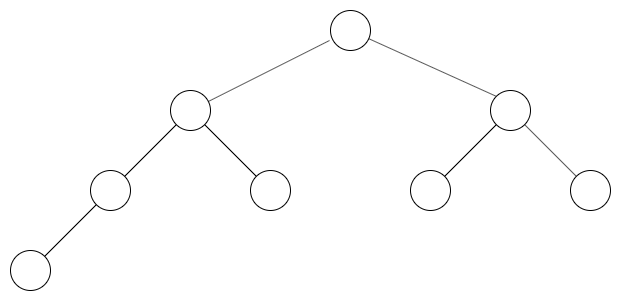
\includegraphics[width=\textwidth]{img/knuth-2.png}
  \caption{Tree drawing generated using Knuth's algorithm.  Such
    drawings contain single node in each column, hence the width is
    maximum}
  \label{fig:knuth_tree}
\end{figure}

Algorithms for tree layout generation confirm to some or all of these
aesthetic requirements. The first tree drawing algorithm developed by
Donald Knuth \cite{Knuth1971} generates drawings that follow the first
three aesthetic rules, but generate drawings that are as wide as the
number of nodes.  Shannon and Wetherell\cite{tidydraw} developed an
improved algorithm that generates trees narrower than the knuth's
algorithm.  Reingold Tilford \cite{reingold} present an algorithm that
generates narrowest possible drawings while confirming to all the
aesthetics.


\vspace{0.5cm}
\begin{table}[H]
  \begin{tabular}{|l|p{9cm}|}
    \hline \textbf{Aesthetic} & \textbf{Description} \\ \hline
    \textit{Parallel Levels} & Nodes of a tree at the same height
    should lie along a straight line, and the straight lines defining
    the levels should be parallel \\ \hline \textit{Relative
      Placement} & In a binary tree, each left child should be placed
    left of its parent and each right child right of its parent
    \\ \hline \textit{Centering} & A parent should be centered over
    its children \\ \hline \textit{Symmetry} & A tree and its mirror
    image should produce drawings that are reflections of one another;
    moreover, a sub-tree should be drawn the same way regardless of
    where it occurs in the tree. \\ \hline
  \end{tabular}
  \caption{List of Aesthetic Requirements for a tree layout}
  \label{table:aesthetics}
\end{table}
\vspace{0.5cm}


\vspace{0.5cm}
\begin{table}[H]
  \begin{tabular}{|c|c|c|c|c|}
    \hline
    \textbf{Aesthetic} & \textbf{Knuth} & \textbf{Wetherell 1} & \textbf{Wetherell 2} & \textbf{Reingold Tilford} \\ \hline
    \textit{Parallel Levels} & True & True & True & True \\ \hline
    \textit{Relative Placement} & True & True & True & True \\ \hline
    \textit{Centering} & True & True & False & True \\ \hline
    \textit{Symmetry} & False & False & False & True \\ \hline  
  \end{tabular}
  \caption{Algorithms and Aesthetics}
  \label{table:algoAesthetics}
\end{table}
\vspace{0.5cm}


The above mentioned aesthetics are some examples of the types of
constraints possible on a layout algorithm.  A different application
may require some other aesthetic or physical constraints.  A different
algorithms would be needed for these constraints.  The process of
developing these algorithms can be simplified by writing partial
programs that define high-level strategies and predicates that define
the constaints. The complete implementation can then be generated
using program synthesis solvers.

\subsubsection{Aesthetics as Constraints}

The aesthetics are encoded as predicates that check if the aesthetic
requirement is satisfied by a given algorithm or not.

For a binary tree, the \textit{parallel levels} aesthetic is described
in equation 2.  This particular implementation assumes that all lines
on which nodes at a level are placed should be horizontal (parallel to
x-axis).  This is a stronger constraint than allowing lines to
parallel at any angle, but for this application, it should be
acceptable because most tree drawings have horizontal level-lines.

\begin{equation}
  \begin{split}
    \forall node, node \in nodeset(tree) \wedge \neg (node.left = null) \wedge \neg (node.right = null)\\
    \Longrightarrow node.left.y = node.right.y
  \end{split}
\end{equation}

\begin{verbatim}
bit parallelLevels(Tree root) {
  if ((root.left != null) && (root.right != null)) {
    if (root.left.y != root.right.y) {
      return false;
    }
    parallelLevels(root.right);
    parallelLevels(root.left);
  }
  return true;
}
\end{verbatim}

The \textit{Relative Placement} aesthetic states that the left child
should be places left of its parent and the right child should be
places right of its parent.  Equation 3 describes this aesthetic.


\begin{equation}
  \begin{split}
    \forall node, node \in nodeset(tree) \\
    \Longrightarrow ((node.left.x < node.x) \wedge (node.x < node.right.x))
  \end{split}
\end{equation}


\begin{verbatim}
bit relativePlacement(Tree root) {
  if (root.left != null) {
    if (root.left.x > root.x || root.left.x == root.x) {
      return false;
    }
    relativePlacement(root.left);
  }  
  if (root.right != null) {
    if (root.right.x < root.x || root.right.x == root.x) {
      return false;
    }
    relativePlacement(root.right); 
  }
  return true;
}
\end{verbatim}


The centering aesthetic is described by equation 4.

\begin{equation}
  \begin{split}
    \forall node, node \in nodeset(tree) \wedge \neg (node.left = null) \wedge \neg (node.right = null)\\
    \Longrightarrow node.x = (node.left.x + node.right.x) / 2
  \end{split}
\end{equation}

\begin{verbatim}
bit centering(Tree root) {
  if ((root.left != null) && (root.right != null)) {
    if (root.center.x != (root.left.x + root.right.x) / 2) {
      return false;
    }
    centering(root.right);
    centering(root.left);
  }
  return true;
}
\end{verbatim}

The predicates described above act as specifications for the layout
program, which is written as a partial program with holes.  Provided
with the partial program and the constraints, the synthesis solver
generates a program which satisfies the given constraints, if any such
solution is possible.

\begin{verbatim}
generator int treeLayout([int N_NODES], TreeNode root,
		int i, int depth, ref int[3] nexts, ref int next_x) {
  if (root == null) {
    return i;
  }
  int j = treeLayout(root.left, i, depth+1, nexts, next_x);
  point = {root.val, {| nexts[depth] | next_x |}, depth};
  root.x = point[0];
  root.y = point[1];
  {| nexts[depth] | next_x |} += 1;
  int k = treeLayout(root.right, j+1, depth+1, nexts, next_x);
  return k;
} 
\end{verbatim}


The above listing describes a partial program that performs inorder
traversal on a tree and assigns x and y values to each node.  Exact
eqauations for assigning x and y coordinates are derived by the
synthesis solver using the constraints.  The constraints which are
defined as predicates can applied to the partial program using
assertions as described below.

\begin{verbatim}
harness void main() {

  // setup ...

  // partial program generator
  treeLayout(root, 0, nexts, next_x);

  // layout constraints
  assert(parallelLevels(root));
  assert(centering(root));
  assert(relativePosition(root));
}
\end{verbatim}


The above specification will generate a layout program that satisfied
the assertions and is derived from the stucture provided in the
partial program.

Im addition to the predicates described above, the solver can also
generate program using input-output examples as constraints.

\section{Conclusion and Future Work}

This report described the application of sketch based program
synthesis to generate data structure layout programs.  A summary of
aesthetics and several algorithms that genrerate tree layouts was
discribed. The method to specify tree layout programs using logical
constraints that is discussed in this report is a basis to develop new
algorithms using some other aesthetics and can be extended to other
data strcutures.

In future work, I plan to use this method to develop an application
where a user can describe the constraints using tree drawings as
examples to generate layouts programs.  An interactive environment
where a user can easily specify the aesthetics should be more useable
than writing predicates and partial programs.  The extent to which the
writing of speficiation and partial programs can be eleminated in
favor of input-output example and what kinds of algorithms can be
generated from them remains to be seen.

\bibliographystyle{unsrt}
\bibliography{references}

\end{document}
